%\documentclass[a4paper,10pt]{article}
%\usepackage[utf8x]{inputenc}


\documentclass[letterpaper,11pt,onecolumn]{article}
\usepackage[margin=1in]{geometry} %one inch margins
\usepackage{amsmath,graphicx}
\usepackage{subcaption}
\usepackage{algorithmic}
\usepackage{algorithm}


\geometry{verbose,margin=1in}

\title{Distributed PageRank - Final Report}
\author{Aaron Myers, Megan Ruthven}

\begin{document}
\maketitle
\tableofcontents
\pagebreak
\section{Introduction}
The purpose of this project is to investigate distributed PageRank by applying Pagerank methods currently in use in the multi-thread case and implement it in the distributed setting. It is to determine if these methods can be scaled to multi-machine systems. We also take a method that has already proven to be effective in the distributed setting and apply it to the Pagerank problem Alternating Direction Method of Multipliers (ADMM) \cite{ADMM}). Immediately below is a more detailed description of each approach. The primary metrics for performace will be: speedup, scalability, and ease of implementation, all of which will be explained in the results section. The last metric is included to suggest that ease of coding and understanding of a method has an impact on the adoption rate in industry and therefore should be included in this investigation.

We chose to investigate ADMM \cite{ADMM} because it would have higher performance for ease of coding and understanding. We applied ADMM to the linear form of the Pagerank problem (Ax=b), but it is more difficult to apply a data-driven approach to the separated minimization problems, so to investigate data-driven approaches outlined in~\cite{Joyce}, we implemented data-driven power iteration with MPI and openMP. Typical power iteration will be refered to as Topology driven. The data-driven methods were Pull, Pull-Push, and Push based. The details of each permutation of the data-driven methods will be discussed in following sections. Because each method is implemented on distributed nodes on a big dataset, each method took advantage of the separate memories, and divided the connection matrices between nodes. There, we implemented a static load balancing regime based on amount of nonzeros in the assigned rows, which proved to be more efficient than load balancing on the number of x elements to calculate. Load balancing will be explained more in the following sections. 

The methods' performance will be compared on total time, speed up, and scalability over varying amount of nodes (MPI), and cores per node (openMP). And finally, we will go over the limitations of the methods in MPI and openMP, and future work. 

\section{Related Work}

Pagerank is the algorithm that Larry Page and Sergey Brin researched, and subsequently used their research to form the company Google. Since then, many researchers have focused on improving different aspects of Pagerank. Our project focused on different implementations of Pagerank to compare and contrast implementations' performance in a distributed setting. 

Iterative solvers for the formulation Ax=b using well known methods including but not limited to: GMRES, BiCGSTAB, CGS, Chebychev iterations, along with Jacobi iteration methods~\cite{FastParallel}. Their results indicated that normal Power Iteration and Jacobi methods almost always performed better than the other linear solvers and although we do not have access to their data sets or machines, we will attempt to generally compare our speedup curves to theirs and expect some correlation. We will also expect that our power iteration and data-driven approaches will perform better than our ADMM solver for Ax=b as they did for \cite{FastParallel}.
 
Previous implementations of Pagerank with MPI~\cite{MPIPR} showed that it is expected for compute time to decrease as the number of MPI processes increase to a certain point. As seen in the figure presented in the paper, with a 1M node graph, after about 30 cores, the solve time starting to trend slightly upward. We assume this increase in solve time is primarily due to the increase in message passing overhead. This would suggest that we should see similar results and also that there may be an optimal core number depending on the size of the data. 

We have worked extremely closely with Joyce Whang as many of our algorithms were taken directly from her research paper and other members of her research group~\cite{Joyce}. In her submitted paper, the algorithms proposed are implemented on a Galois multithread system. Our data-driven implementations are taken directly from her paper and implemented with the MPI and openMP frameworks. This extraction to the distrubuted setting is to confirm or deny the idea that her algorithms could also be effective across nodes.

\section{Load Balancing}
Before this paper details the different algorithms we implemented, it will talk about load balancing. Load balancing on distributed systems could be scheduled in task or job manner, as discussed in~\cite{distributed}, where jobs were a collection of tasks. Because MPI is best suited for batch passing of messages, our project used a job based approach. The two approaches were to balance jobs by number of tasks (indices to compute Pagerank), or balance by total average work for each node (summation of nonzeros of each incoming node for the assigned indices). First we implemented our methods where each node had the same amount of tasks to compute. Then, we implemented balancing by total work, and compared the differences. The topological and data-driven Pagerank algorithms consistantly sped up where the total work balancing was about two times faster than the balanced tasked method. For these reasons, the results reflect algorithms which used the work balancing method. 

\section{Algorithms and Implementation}

This section discusses the implementations of different methods for computing pagerank. This includes topological, data-driven, and ADMM Pagerank. 

\subsection{Topology-driven}
This is the classic implmentation for calculating Pagerank, seen in algorithm~\ref{alg:top} . It is straight forward, but recalculates all X values every iteration. This could be redundant on a large percentage of the X indices, and therefore, it could waste computational power. 

\begin{algorithm}
\caption{Topology-driven Pagerank}
\label{alg:top}
\begin{algorithmic}[1]
  \STATE Input: graph $P_{r} = (V_r, E_r)$, $\alpha$, $\epsilon$
  \STATE Output: Pagerank $\mathbf{x}$
  \STATE Initialize $\mathbf{x} = \alpha \mathbf{e}$
  \STATE $\exists  \medspace \mathbf{x_r}$ in $\mathbf{x}$ as $P_r$ is to $P$
  \WHILE{true}
	\FOR{$v \in V_r$}
		\STATE $x_{v}^{(k+1)} = \alpha + (1 - \alpha) \sum_{w \in S_v} \frac{x_{w}^{(k)}}{|T_w|} $
		\STATE $\delta_{v} = | x_{v}^{(k+1)} - x_{v}^{(k)} | $
	\ENDFOR
	\STATE sync all $\mathbf{x_r}$ between nodes
	\IF{$\|\delta \|_{\infty} < \epsilon$}
		\STATE break;
	\ENDIF
  \ENDWHILE
  \STATE $\mathbf{x} = \frac{\mathbf{x} }{\|x\|_{1}}$
\end{algorithmic}
\end{algorithm}

In the topological algorithm, every $x_v$ is updated. Each node computes a subsection of $\mathbf{x}$, named $\mathbf{x_r}$, then all of the nodes combine their new result in batch to create a new $\mathbf{x}$ in order to continue to compute the newer values of $\mathbf{x_r}$. All of the recomputation within each node only updates the current $x_v$, this creates for a thread safe algorithm.

\subsection{Data-Driven Pagerank}
In addition to the ADMM implementation, we implemented power iteration, as well as three permutations of the data-driven pagerank method (pull, pull-push, and push). The data-driven method (taken from \cite{Joyce}) aims to minimize unnecessary computation by only updating pageranks of elements whose incoming connections were upated to a satisfactory degree. 

\begin{algorithm}
\caption{Pull Data-driven Pagerank}
\label{alg:pull}
\begin{algorithmic}[1]
  \STATE Input: graph $P_{c} = (V_c, E_c)$, $\alpha$, $\epsilon$
  \STATE Output: Pagerank $\mathbf{x}$
  \STATE Initialize $\mathbf{x} = \alpha \mathbf{e}$ and $\mathbf{t_c} = true \times \mathbf{e_c}$
  \STATE $\exists  \medspace \mathbf{x_c}$ in $\mathbf{x}$ as $P_c$ is to $P$
  \WHILE{$\exists \medspace v \medspace s.t. \medspace t_v = true$}
	\STATE $t^{new} = false \times \mathbf{e}$
	\FOR{$v \in V_c$}
		\IF{$t_v = true$}
			\STATE $x_{v}^{new} = \alpha + (1 - \alpha) \sum_{w \in S_v} \frac{x_{w}}{|T_w|} $
			\IF{ $| x_{v}^{new} - x_{v} | \geq \epsilon  $}
				\STATE $x_v = x_v^{new}$
				\FOR{$w \in T_v$}
					\STATE $t_w^{new} = true$
				\ENDFOR
			\ENDIF
		\ENDIF
	\ENDFOR
	\STATE sync all $\mathbf{x_c}$ between nodes
	\STATE logical or all $t = t^{new}$ between nodes
  \ENDWHILE
  \STATE $\mathbf{x} = \frac{\mathbf{x} }{\|x\|_{1}}$
\end{algorithmic}
\end{algorithm}


The Pull data-driven method in algorithm~\ref{alg:pull} selectively updates the values of $x_v$ based on if an incoming connected node updated itself above the threshold, $\epsilon$. This is determined by the array $t_c$, which is a set of $c$ indices for that node. In the computation of $x_v$, if the difference between the new and old value is above $\epsilon$, set all outgoing nodes' $t_w$ to true. Notice that each element, $v$, updates its value, $x_v$, and indices of $t$ both in and out of set $c$. This requires the syncing of all copies of $t^{new}$ between nodes with a logical or. Additionally, this algorithm accesses more memory by accessing incoming nodes' pagerank and outgoing nodes' $t^{new}$.

\begin{algorithm}
\caption{Pull-Push Data-driven Pagerank}
\label{alg:pullpush}
\begin{algorithmic}[1]
  \STATE Input: graph $P_{c} = (V_c, E_c)$, $\alpha$, $\epsilon$
  \STATE Output: Pagerank $\mathbf{x}$
  \STATE Initialize $\mathbf{x} = \alpha \mathbf{e}$
  \STATE $\exists  \medspace \mathbf{x_c}$ in $\mathbf{x}$ as $P_c$ is to $P$
  \STATE Initialize $\mathbf{r} = \mathbf{0}$
  \FOR{$v \in V_c$}
	\FOR{$w \in S_v$}
		\STATE $r_v = r_v + \frac{1}{|T_w|}$
	\ENDFOR
	\STATE $r_v = (1 - \alpha)\alpha r_v$
  \ENDFOR
  \WHILE{$\exists \medspace v \medspace s.t. \medspace r_v \geq \epsilon$}
	\STATE $r^{new} = \mathbf{0}$
	\FOR{$v \in V_c$}
		\IF{$r_v \geq \epsilon$}
			\STATE $x_{v} = \alpha + (1 - \alpha) \sum_{w \in S_v} \frac{x_{w}}{|T_w|} $
			\FOR{$w \in T_v$}
				\STATE $r_w^{new} = r_w^{new} + \frac{r_v \alpha}{|T_v|}$
			\ENDFOR
		\ELSE
			\STATE $r_v^{new} = r_v^{new} + r_v$
		\ENDIF
	\ENDFOR
	\STATE sync all $\mathbf{x_c}$ between nodes
	\STATE add all and scatter $ r_c = r^{new}$ between nodes
  \ENDWHILE
  \STATE $\mathbf{x} = \frac{\mathbf{x} }{\|x\|_{1}}$
\end{algorithmic}
\end{algorithm}

The Pull-Push data-driven method in algorithm~\ref{alg:pullpush} selectively updates the values of $x_v$ based on if its residual is above a threshold, $\epsilon$. The residuals are accounted for in the $\mathbf{r}$ vector and batch updated to transfer residual values between nodes. Notice that each element, $v$, updates its value, $x_v$, and indices of $r$ both in and out of set $c$. This requires the syncing of all copies of $r^{new}$ between nodes by summing. Additionally, this algorithm accesses more memory by accessing incoming nodes' pagerank and outgoing nodes' $r^{new}$.

\begin{algorithm}
\caption{Push Data-driven Pagerank}
\label{alg:push}
\begin{algorithmic}[1]
  \STATE Input: graph $P_{c} = (V_c, E_c)$, $\alpha$, $\epsilon$
  \STATE Output: Pagerank $\mathbf{x}$
  \STATE Initialize $\mathbf{x} = \alpha \mathbf{e}$
  \STATE $\exists  \medspace \mathbf{x_c}$ in $\mathbf{x}$ as $P_c$ is to $P$
  \STATE Initialize $\mathbf{r} = \mathbf{0}$
  \FOR{$v \in V_c$}
	\FOR{$w \in S_v$}
		\STATE $r_v = r_v + \frac{1}{|T_w|}$
	\ENDFOR
	\STATE $r_v = (1 - \alpha)\alpha r_v$
  \ENDFOR
  \WHILE{$\exists \medspace v \medspace s.t. \medspace r_v \geq \epsilon$}
	\STATE $r^{new} = \mathbf{0}$
	\FOR{$v \in V_c$}
		\IF{$r_v \geq \epsilon$}
			\STATE $x_{v} = x_{v} + r_v $
			\FOR{$w \in T_v$}
				\STATE $r_w^{new} = r_w^{new} + \frac{r_v \alpha}{|T_v|}$
			\ENDFOR
		\ELSE
			\STATE $r_v^{new} = r_v^{new} + r_v$
		\ENDIF
	\ENDFOR
	\STATE add all and scatter $ r_c = r^{new}$ between nodes
  \ENDWHILE
\STATE sync all $\mathbf{x_c}$ between nodes
  \STATE $\mathbf{x} = \frac{\mathbf{x} }{\|x\|_{1}}$
\end{algorithmic}
\end{algorithm}

The Push data-driven method in algorithm~\ref{alg:push} selectively updates the values of $x_v$ based on if its residual is above a threshold, $\epsilon$. It updates $x_v$ by only using $r_v$. This accesses less memory by bypassing fetching all of the incoming nodes current values $x_w$. The residuals are accounted for in the $\mathbf{r}$ vector and batch updated to transfer residual values between nodes. Notice that each element, $v$, updates its value, $x_v$, and indices of $r$ both in and out of set $c$. This requires the syncing of all copies of $r^{new}$ between nodes by summing. 

Although MPI allowed for a distributed Pagerank algorithm, there were a couple of restrictions on the implementation because of the MPI and openMP framework we chose to use. When syncing values between nodes, MPI requires all nodes to simultaneously request and send the information they require. This means that all of the independent nodes have to update the values in batch. The original implementation in Galois~\cite{Joyce} utilized the asynchronisity of value updates unique to Galois to be able to have threadsafe updates, and shared residual values between threads. This is not a feature in openMP or MPI. In openMP, each thread kept track of its own residuals for the whole set of indices, and reduced after all were calculated within each node, then shared its values to sum up all of the nodes' residual values. These 2 steps of synchronization were not necessary in the Galois implementation. Additionally, the batch update of residuals and the boolean update vector meant that a meaningful worklist was impossible to keep without the vectors from the other nodes. This meant, to selectively compute a new value the Pagerank, each node had to go through each value of the residual or update vectors to check if it met the standards of update. 

The new vectors of information about each index needed to be passed between nodes. More information to send corresponds with a longer amount of time spend on sending data. In the case of algorithms~\ref{alg:pull} and~\ref{alg:pullpush}, they both send $\mathbf{x_c}$ and an update vector. This does not scale well for big 

NOTE: THIS NEEDS MORE INFORMATION 

\subsection{Linear System Approach: Ax=b Formulation}
This approach requires that we form the Pagerank problem into a different linear system (Ax=b) where we fundamentally look at methods of iterating or directly solving for an inverse to solve for x which would would provide the list of Pagerank values. Below is a simple derivation taken from \cite{FastParallel}.
\begin{center}
\begin{align}
	P' &= P + dv^{T} \\
	P'' &= cP' + (1-c)ev^{T} \\
	x^{k+1} &= P''^{T}x^{k}
\end{align}

\end{center}
Where P$'$ and P$''$ are the modified PageRank matrices that have the modifications necessary to create a connected graph and add a personalization factor and e is a vector of all 1's, resulting in equation 3, the Power Iteration approach to Pagerank.
\newline
\linebreak
Given the additional information below, we can derive the linear system for Pagerank.


\begin{center}
\begin{align}
  e^{T}x & = x^{T}e = \|x\|_{1} = \|x\| \\
  d^{T}x &= \| x\| - \| P^{T}x\| \\
  x &= [cP^{T} + c(vd^{T}) + (1-c)ve^{T}]x
\end{align}
\end{center}

Combining the information above, we arrive at the following equation:

\begin{center}
\begin{equation}
  (I-cP^{T})x = kv
\end{equation}
\end{center}
We now have Pagerank in a linear form (Ax=b), where A = I-c$P^{T}$ and kv = b. If in addition, we normalize x, we have the following:

\begin{center}
  \begin{align}
	k &= \|x\| - c \|P^{T}x\| = (1-c) \|x\| + d^{T}x \\	
	k &= 1-c 
  \end{align}
\end{center}



\subsection{ADMM}

Many of the articles we encountered for solving parallel pagerank in the linear form used Jacobi iteration or some Krylov Subspace method (GMRES, BiCGSTAB, etc), but we attempted to implement something we were introduce to in this course, namely ADMM \cite{ADMM}. This is an extremely simple way to parallelize a linear solve. This process attempts to split the linear problem into subsections, solve separately, and combine the information in a very specific way. 
We will compare these results to the implementation of GMRES (Generalized Minimal RESidual method) and BiCGSTAB (BiConjugate Gradient method with STABilization) for the same problem parallelizing using PETSc (a software with great tools for parallizing linear solvers) \cite{Power Law Graphs}. We expect ADMM to have worse performance, measured by speedup, but we would like to quantify the loss in accuracy/time relative to the ease of implementation and scalability.
\newline
\linebreak
Below is a brief description of the ADMM idea and algorithm \cite{ADMM}.
\newline
We take the linear problem and split up the data accordingly:
\begin{center}
\begin{align}
	A &= \left[ A_{1} ... A_{n} \right]' \\
	b &= \left[ b_{1} ... b_{n} \right]' 
\end{align}
\end{center}
Our origninal minimization of Ax-b with a certain norm and regulariztion on x now becomes:

\begin{center}
\begin{align}
	&minimize \: \: \: \sum_{i=1}^{N} l_{i}(A_{i}x_{i} - b_{i}) + r(z) \\
	&subject \: \: \: to \: \: \: x_{i} - z = 0 \: \: \: \forall i
\end{align}
\end{center}
Where $x_{i}$ are local variables that we force to match the global solution z at each step and N is the number of processes used to solve the problem. This method also includes an 'augmented lagragian' term. This term is used to bring robustness to the dual ascent problem and result in convergence without criteria like strict convexity or finiteness of the function. This is discussed in much greater detail in \cite{ADMM}. Below is the augemented lagrangian which is used to derive the resulting algorithm.
\newline
\begin{center}
  \begin{align}
		L_{\rho}(x,y) &= f(x) + y^{T}(Ax-b) + \frac{\rho}{2}\|Ax - b\|_{2}^{2} \\
  \end{align}
\end{center}


The resulting algorithm, using the augmented lagrangian presented in the ADMM method \cite{ADMM}, is as follows:

\begin{center}
\begin{algorithm}
\caption{ADMM Iteration}
\begin{algorithmic}[1]
	\STATE $x_{i}^{k+1} = argmin_{x} \: \: \: l_{i}(A_{i}x_{i} - b_{i}) + \frac{\rho}{2} \| x_{i}^{k} - z^{k} - u_{i}^{k} \|_{2}^{2}$ 
	\STATE $z^{k+1} = argmin_{z} \: \: \: r(z) + \frac{N \rho}{x} \| z^{k} - \bar{x}^{k+1} - \bar{u}^{k} \|_{2}^{2} $
	\STATE $u_{i}^{k+1} = u_{i}^{k} + x_{i}^{k+1} - z^{k+1} $ 
  \end{algorithmic}
\end{algorithm}
\end{center}

Where $u_{i}^{k} = \frac{1}{\rho} y_{i}^{k}$ and for our implementation, we chose the $L^{1}$ regularization term (also known as lasso) with a gradient descent sovler and we also attempted a direct solve with Eigen for the minimization for x, although the results were poor. Using the lasso regulariztion the z update becomes soft-thresholding update. Considering the Lasso method, the updated algorithm is below.

\begin{center}
\begin{algorithm}
\caption{ADMM Iteration with Lasso}
\begin{algorithmic}[1]
  \STATE $x_{i}^{k+1} = argmin_{x} \: \: \: \|(A_{i}x_{i} - b_{i})\|_{2}^{2} + \frac{\rho}{2} \| x_{i}^{k} - z^{k} - u_{i}^{k} \|_{2}^{2}$ 
  \STATE $z^{k+1} = S_{\lambda/\rho N} (\bar{x}^{k+1} - \bar{u}^{k})$
	\STATE $u_{i}^{k+1} = u_{i}^{k} + x_{i}^{k+1} - z^{k+1} $ 
  \end{algorithmic}
\end{algorithm}
\end{center}

Where S is defined componend-wise in the following way:
\begin{center}
	\begin{equation}
	  S_{\lambda/\rho N}(x_{i}) := (x_{i} - \frac{\lambda}{\rho N})_{+} - (-x_{i} - \frac{\lambda}{\rho N})_{+}
	\end{equation}
\end{center}


The first approach we took to solving the minimization problem on each separate process was to use the direct inversion with Eigen. Below is the resulting equation required to be solved for direct inversion.
\begin{center}
  \begin{equation}
	x^{k+1} := (A_{i}^{T}A_{i} + \rho I)^{-1}(A_{i}^{T}b_{i} + \rho(z^{k} - u_{i}^{k}))
	\label{}
  \end{equation}
\end{center}
The above equation makes it clear that using this direct solve method would require the formation of an mxm matrix (the same size as the original matrix) which would then be dense. This renders the direct solve method nearly usesless and indeed when attempting this method, the algorithm (on a small matrix, m=1770961) took 2 hours to complete 1 iteration.
\newline
\linebreak
Another method we investigated is the gradient descent algorithm. Below is a short description of gradient descent for those unfamiliar with the method.

\begin{center}
  \begin{algorithm}
	\caption{Gradient Descent Algorithm}
	\begin{algorithmic}[1]
	  \STATE Set Threshold
	  \STATE Initialize $x_{n+1}, x_{n}$ s.t. $\|x_{n+1} - x_{n}\| > threshold$
	  \WHILE{$\|x_{n+i1} - x_{n}\| > threshold$}
	  \STATE $x_{n+1} = x_{n} - \alpha \nabla F(x_{n})$
	  \STATE select $\alpha$  s.t. $\alpha$ = min $\nabla F(x_{n+1})$
	  \ENDWHILE
	\end{algorithmic}
  \end{algorithm}
\end{center}
Step 5 above is done with line search looking at a set of discrete values between 0.001 and 10.

\section{Datasets}
In order to compare performances of the algorithms in different conditions, five datasets were used. They vary in size, sparsity, and quality of symmetry. These qualities are displayed in table~\ref{table:data}. All of these qualities influence the performance of the algorithms. The PLD, Twitter RV, and SD1 datasets were the same ones used in~\cite{Joyce}. They are good examples of fairly sizeable datasets that 

\begin{center}
  \begin{tabular}{ c | c  | c | c }
    \hline
    Name & Size & Indices & Symmetric \\ \hline \hline
    Livejournal & 1.1 GB & 1,770,961 & Yes \\ \hline
    Friendster & 7 GB & 15,853,098 & Yes \\ \hline
    PLD & 10.4 GB & 39,497,202 & No \\ \hline
    Twitter RV & 23.5 GB & 41,652,230 & No \\ \hline
    SD1 & 32.7 GB & 82,924,685 & No \\
    \hline
  \end{tabular}
  \label{table:data}
\end{center}



\section{Results}
The different methods had varying quantitative and qualitative results. These included the time to complete, speedup, scalability, and ease of coding. 

\subsection{Power Iteration Results}

The Topology and Data-driven Pagerank implementations were written in C++ and used MPI to run on distributed nodes, and openMP to run multiple threads within each node. Each algorithm’s performance was timed on each of the datasets in all of the combinations of 1, 4, 8, 16, 32 compute nodes and 1, 4, 8, and 16 threads. For additional understanding of how performance changed over number of nodes and threads, scalability and speedup are visualized in figures~\ref{fig:time}. These measures are the same measures used in~\cite{Joyce}. 

\begin{center}
  \begin{equation}
	Scalability = \frac{run-time \ of \ method \ m \ with \ a \ single \ thread}{run-time \ of \ method \ m \ with \ t \ threads}
	\label{math:scale}
  \end{equation}
\end{center}

\begin{center}
  \begin{equation}
	Speedup = \frac{run-time \ of \ the \ fastest \ single-thread \ method}{run-time \ of \ method \ m \ with \ t \ threads}
	\label{math:speed}
  \end{equation}
\end{center}

Scalability,~\ref{math:scale}, is a metric to show the change in runtime from one method’s baseline, whereas speedup,~\ref{math:speed}, is to show the change in runtime from the best case scenario method at baseline configuration. Both frameworks have different artifacts that enable or hinder speedup and scalability as the number of threads increase. So, speedup and scalability are evaluated for MPI and openMP separately. 

\begin{figure}
\begin{subfigure}{.33\textwidth}
  \centering
  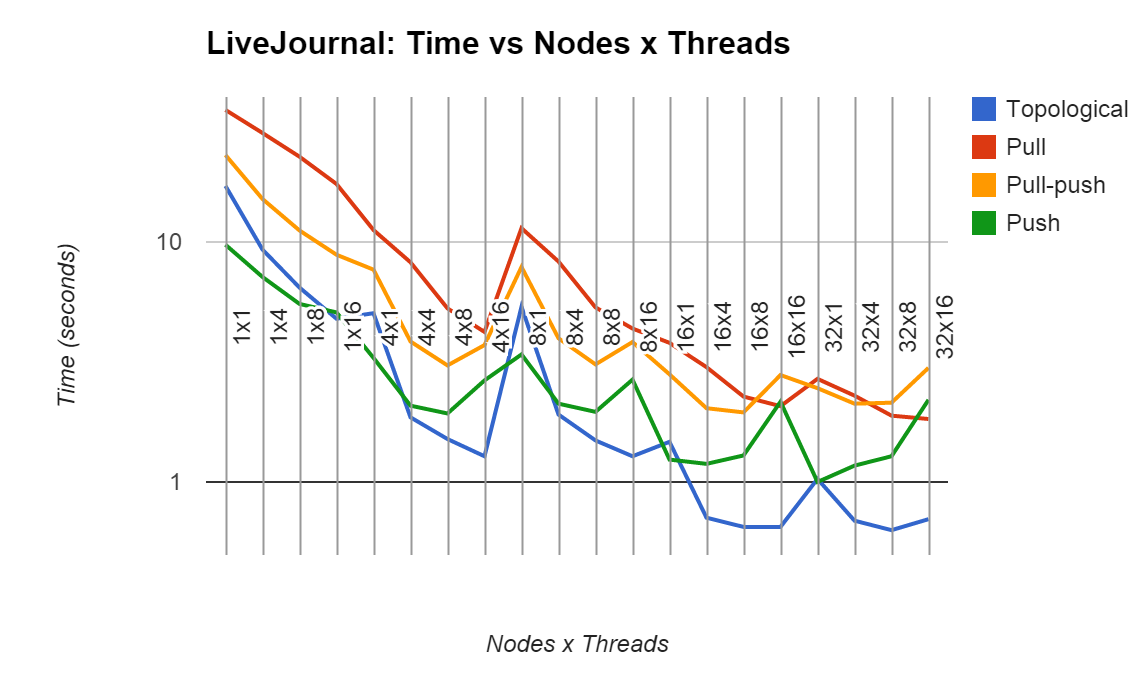
\includegraphics[width=.99\linewidth]{LiveJournalTime}
  \caption{Live Journal}
  \label{fig:lgtime}
\end{subfigure}%
\begin{subfigure}{.33\textwidth}
  \centering
  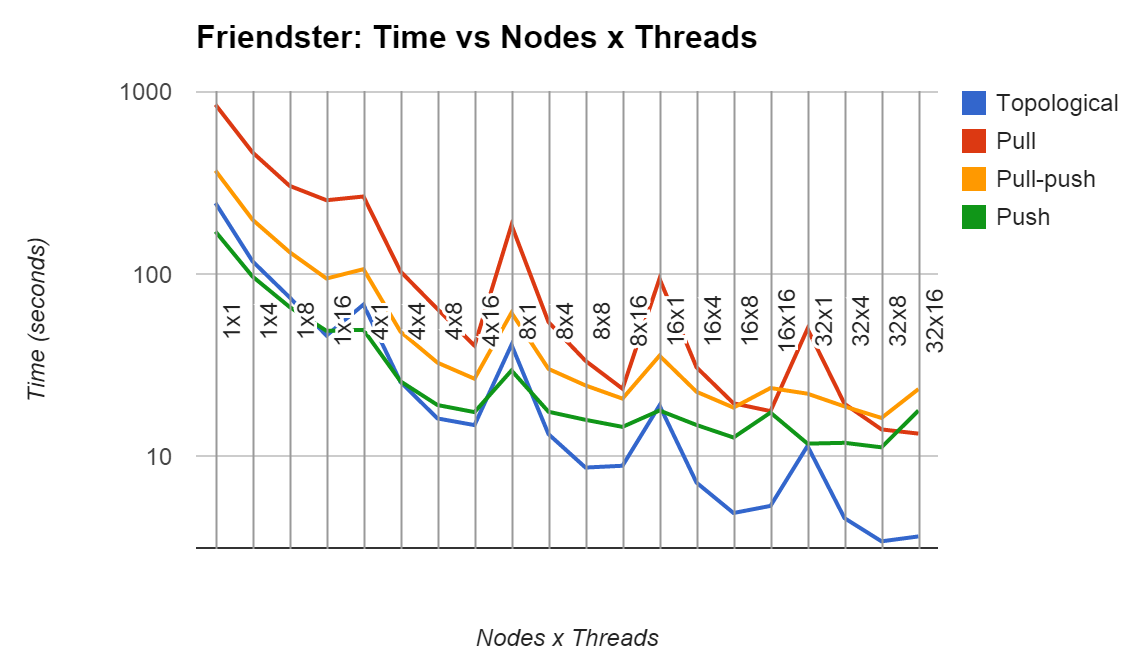
\includegraphics[width=.99\linewidth]{FriendsterTime}
  \caption{Friendster}
  \label{fig:ftime}
\end{subfigure}
\begin{subfigure}{.33\textwidth}
  \centering
  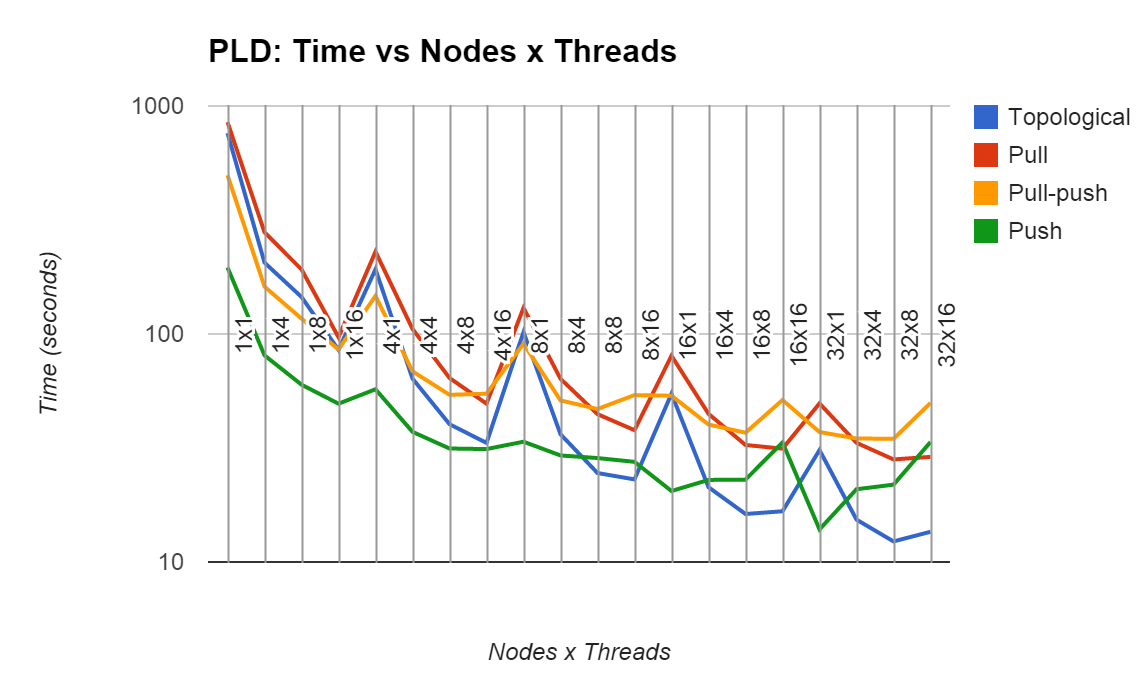
\includegraphics[width=.99\linewidth]{PLDTime}
  \caption{PLD}
  \label{fig:ftime}
\end{subfigure}
\caption{Convergence times of different PageRank implementations on datasets from table~\ref{table:data}}
\label{fig:time}
\end{figure}

\begin{figure}
\begin{subfigure}{.33\textwidth}
  \centering
  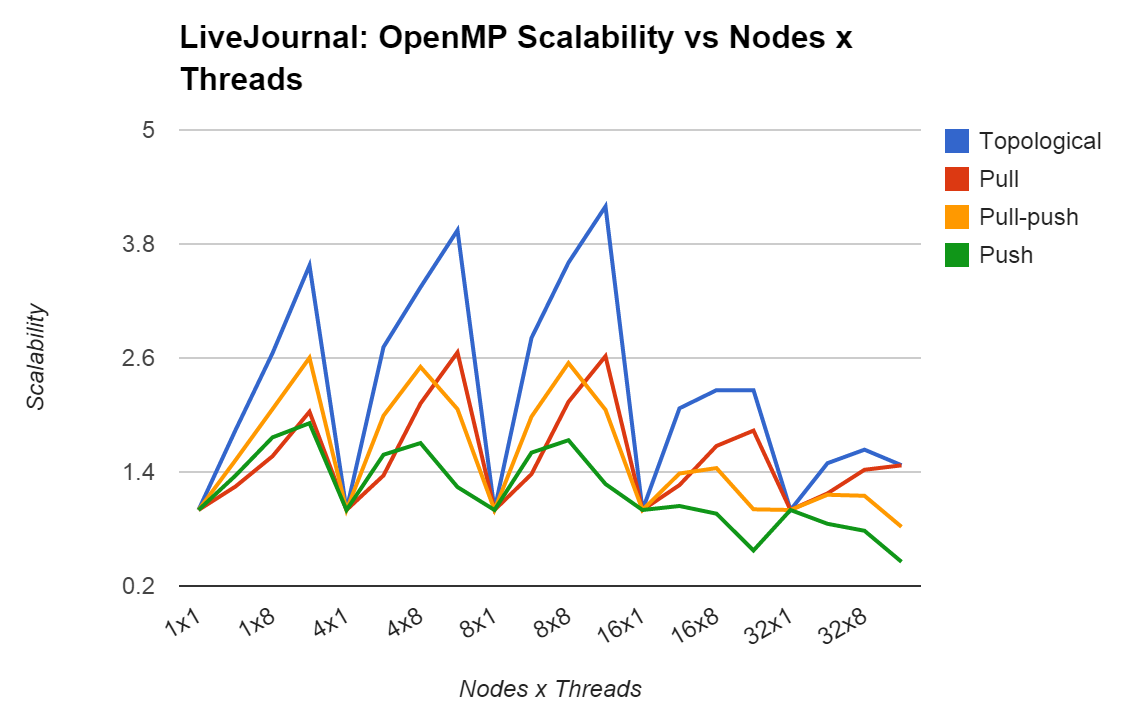
\includegraphics[width=.99\linewidth]{LiveJournalOMPScalability}
  \caption{Live Journal}
  \label{fig:lgtime}
\end{subfigure}%
\begin{subfigure}{.33\textwidth}
  \centering
  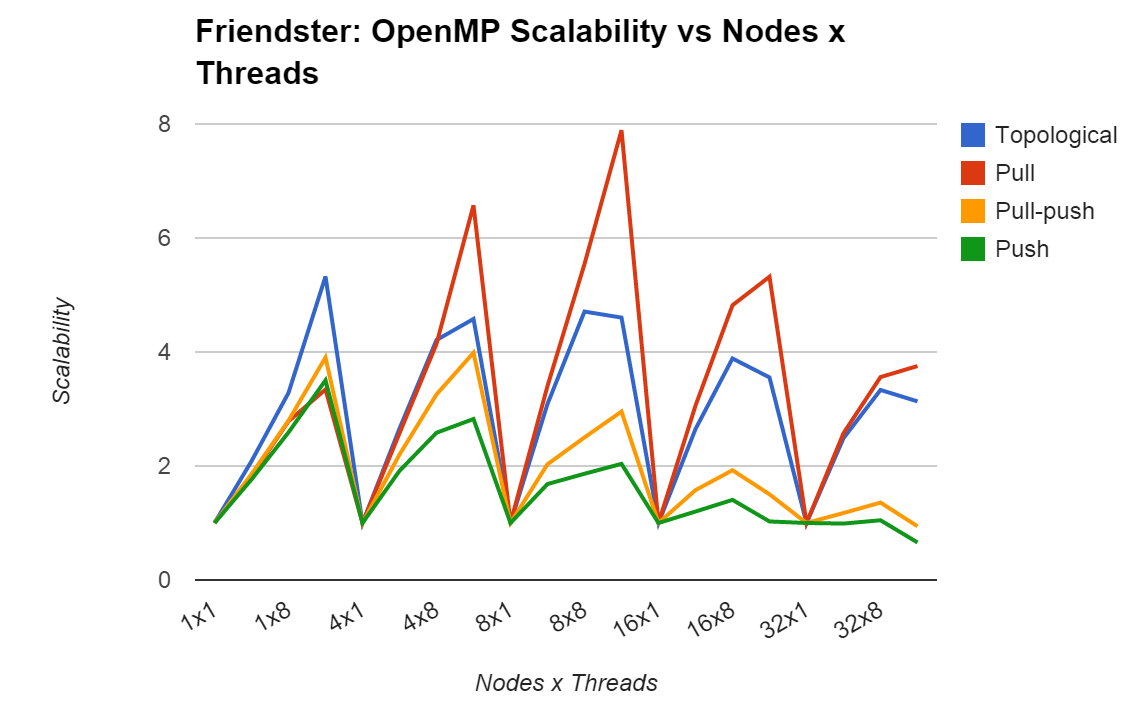
\includegraphics[width=.99\linewidth]{FriendsterOMPScalabilty}
  \caption{Friendster}
  \label{fig:ftime}
\end{subfigure}
\begin{subfigure}{.33\textwidth}
  \centering
  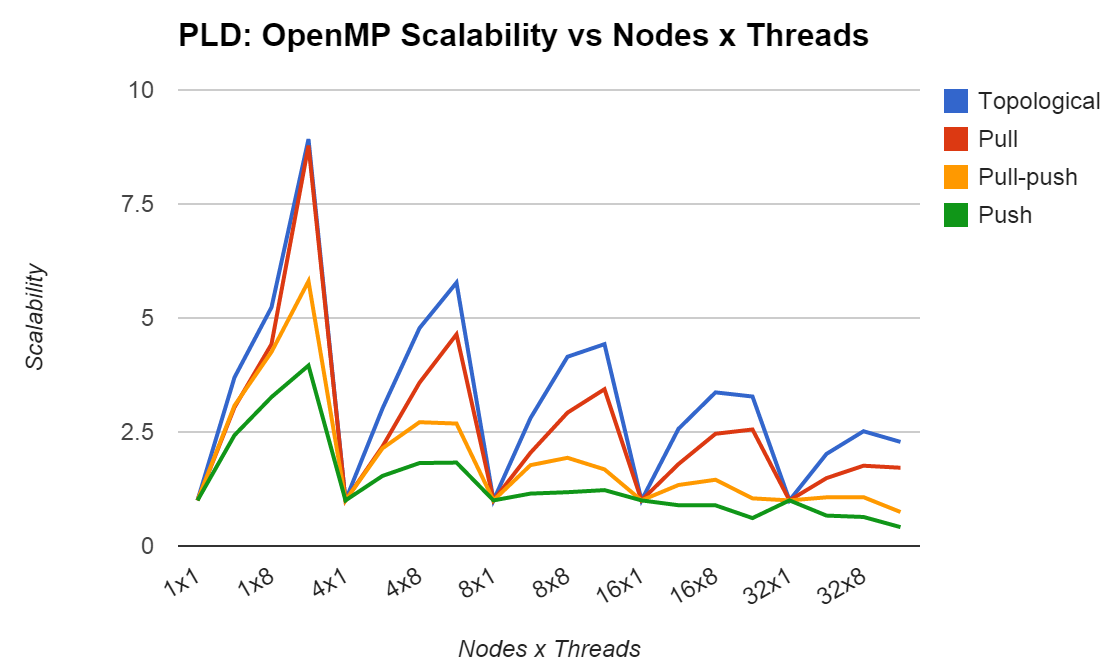
\includegraphics[width=.99\linewidth]{PLDOMPScalability}
  \caption{PLD}
  \label{fig:ftime}
\end{subfigure}
\caption{Scalability over openMP threads of different PageRank implementations on datasets from table~\ref{table:data}}
\label{fig:scOMP}
\end{figure}

\begin{figure}
\begin{subfigure}{.33\textwidth}
  \centering
  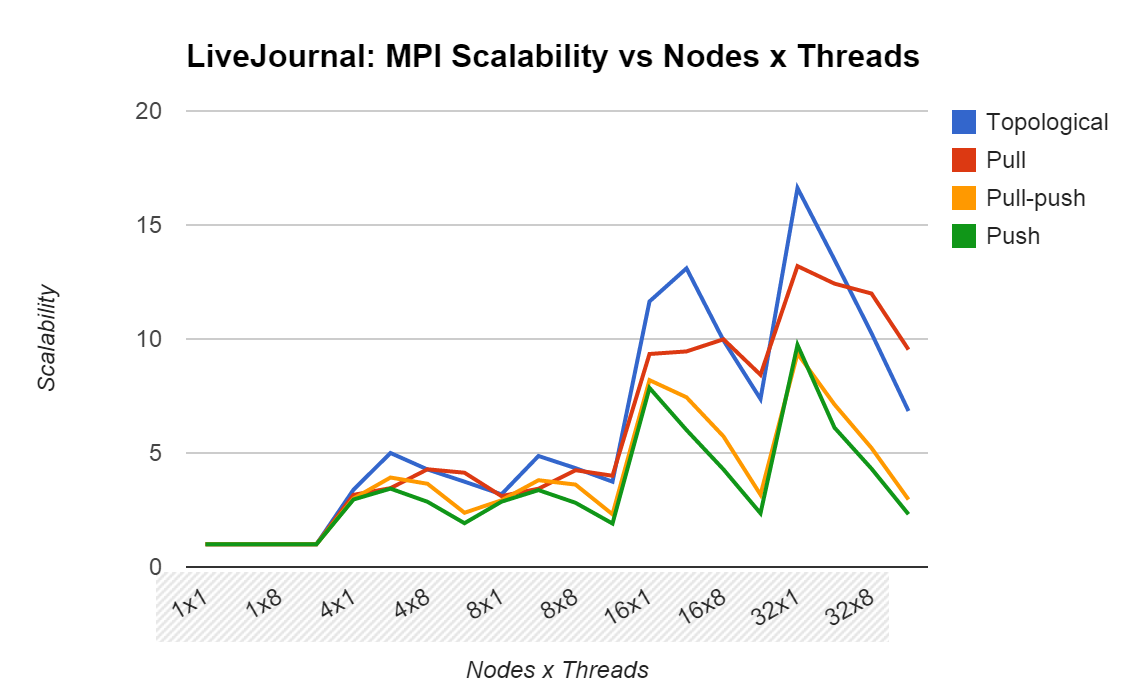
\includegraphics[width=.99\linewidth]{LiveJournalMPIScalability}
  \caption{Live Journal}
  \label{fig:lgtime}
\end{subfigure}%
\begin{subfigure}{.33\textwidth}
  \centering
  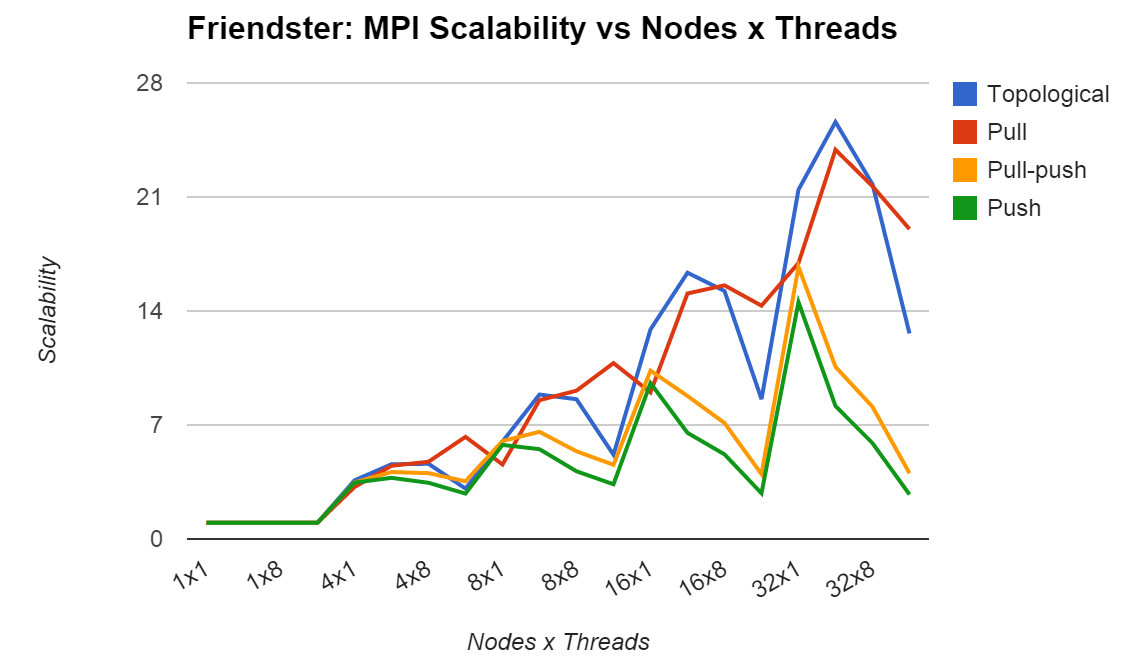
\includegraphics[width=.99\linewidth]{FriendsterMPIScalability}
  \caption{Friendster}
  \label{fig:ftime}
\end{subfigure}
\begin{subfigure}{.33\textwidth}
  \centering
  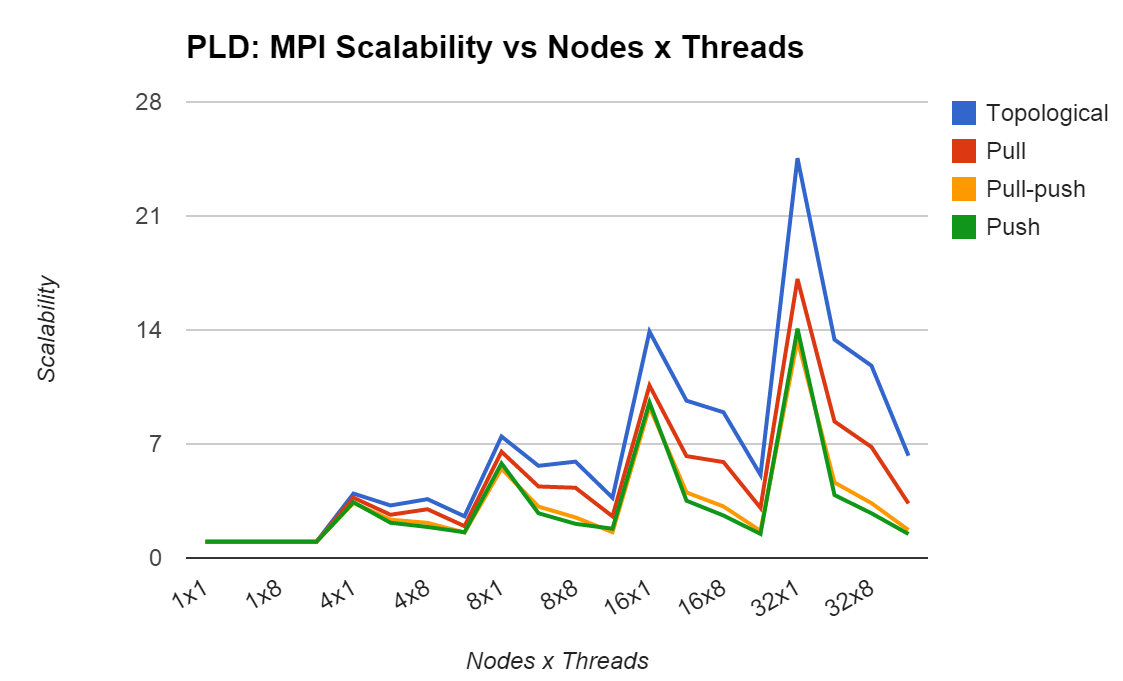
\includegraphics[width=.99\linewidth]{PLDMPIScalability}
  \caption{PLD}
  \label{fig:ftime}
\end{subfigure}
\caption{Scalability over MPI nodes of different PageRank implementations on datasets from table~\ref{table:data}}
\label{fig:scMPI}
\end{figure}

\begin{figure}
\begin{subfigure}{.33\textwidth}
  \centering
  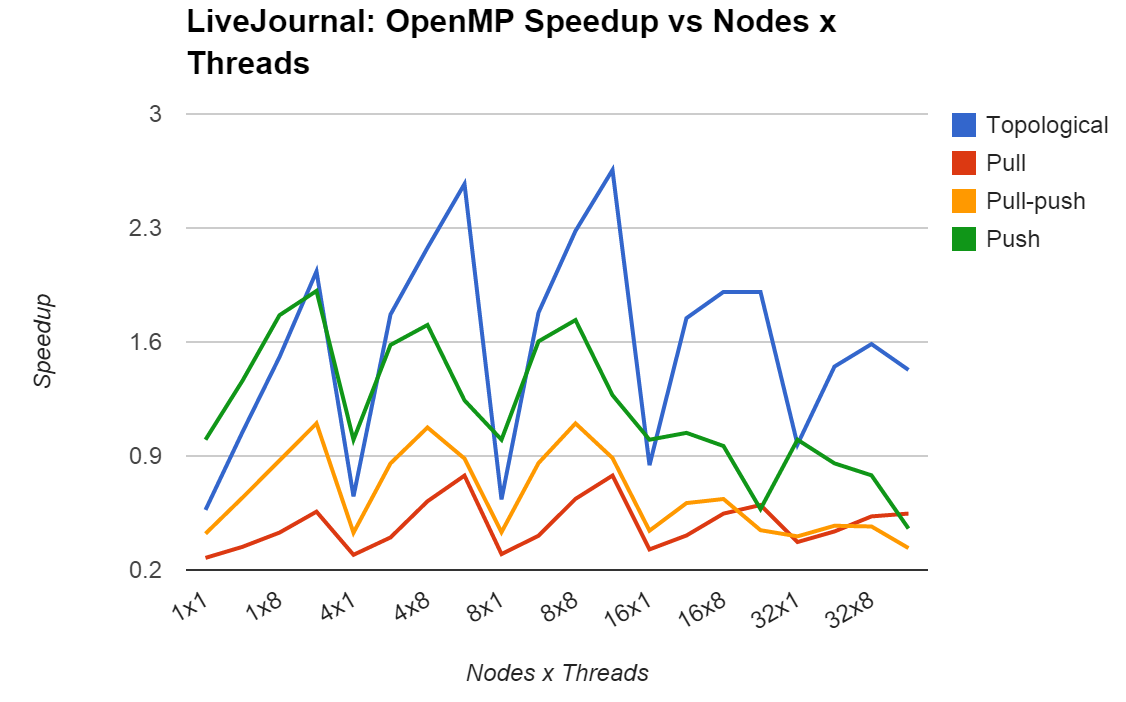
\includegraphics[width=.99\linewidth]{LiveJournalOMPSpeedup}
  \caption{Live Journal}
  \label{fig:lgtime}
\end{subfigure}%
\begin{subfigure}{.33\textwidth}
  \centering
  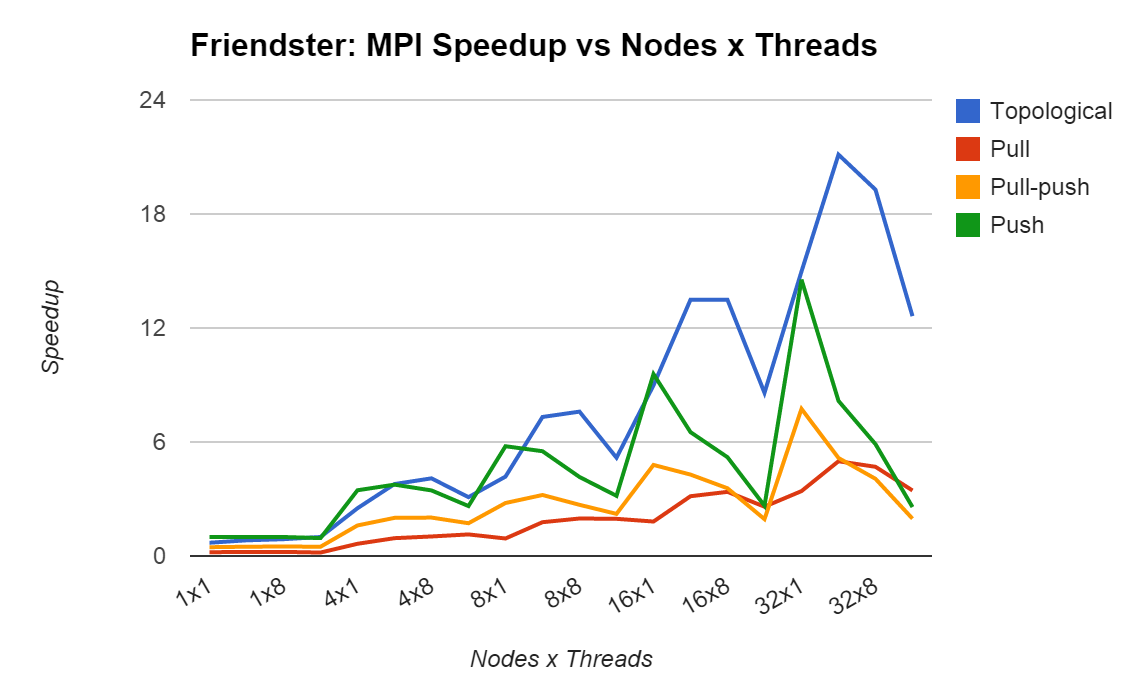
\includegraphics[width=.99\linewidth]{FriendsterMPISpeedup}
  \caption{Friendster}
  \label{fig:ftime}
\end{subfigure}
\begin{subfigure}{.33\textwidth}
  \centering
  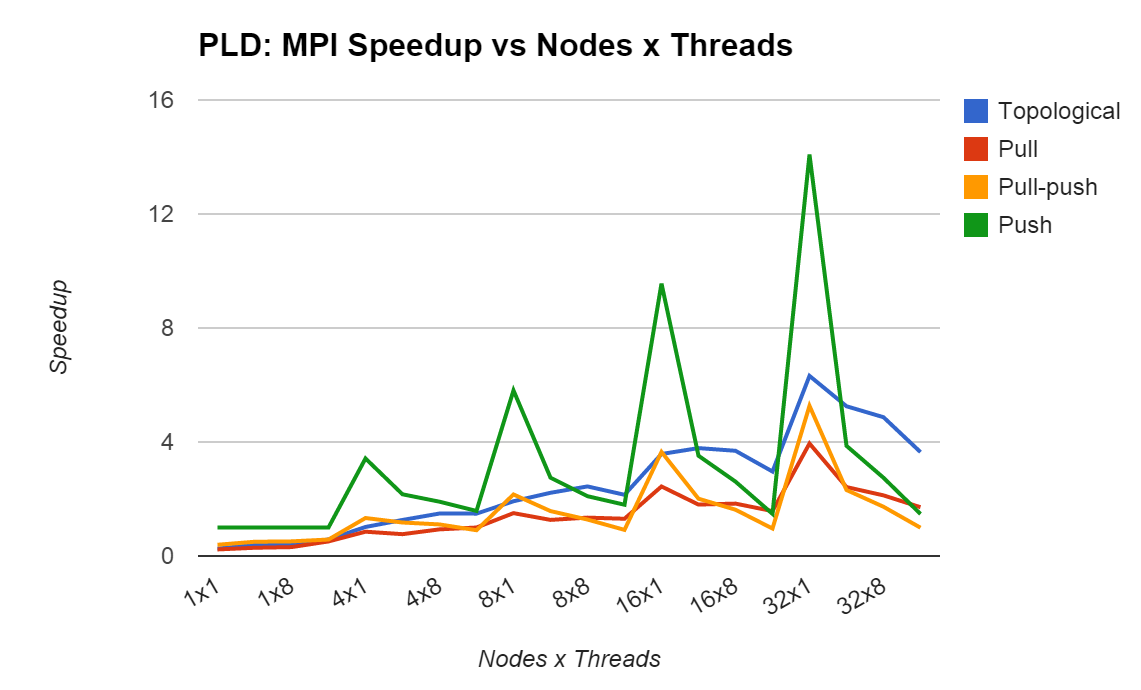
\includegraphics[width=.99\linewidth]{PLDMPISpeedup}
  \caption{PLD}
  \label{fig:ftime}
\end{subfigure}
\caption{Speedup over openMP threads of different PageRank implementations on datasets from table~\ref{table:data}}
\label{fig:spOMP}
\end{figure}

\begin{figure}
\begin{subfigure}{.33\textwidth}
  \centering
  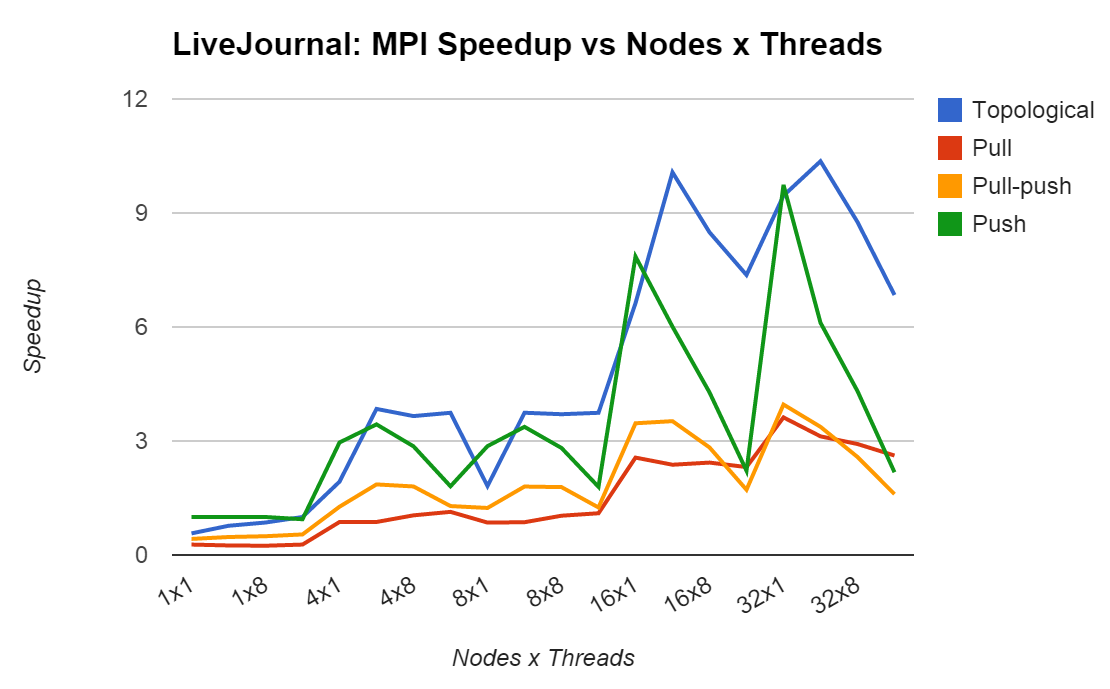
\includegraphics[width=.99\linewidth]{LiveJournalMPISpeedup}
  \caption{Live Journal}
  \label{fig:lgtime}
\end{subfigure}%
\begin{subfigure}{.33\textwidth}
  \centering
  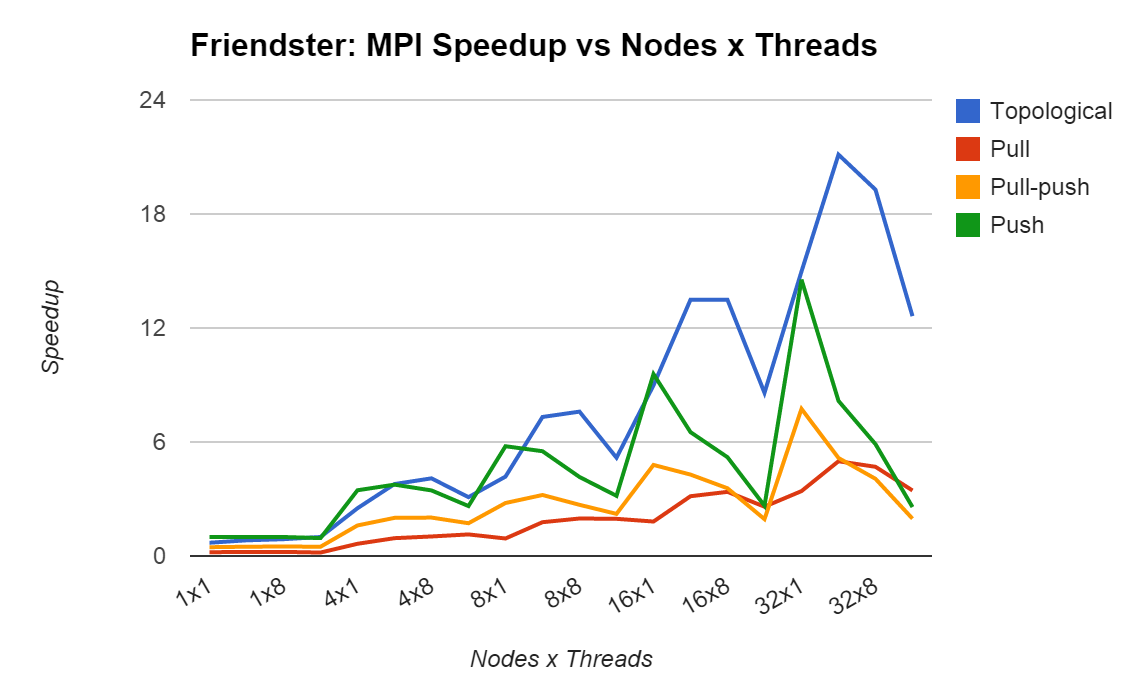
\includegraphics[width=.99\linewidth]{FriendsterMPISpeedup}
  \caption{Friendster}
  \label{fig:ftime}
\end{subfigure}
\begin{subfigure}{.33\textwidth}
  \centering
  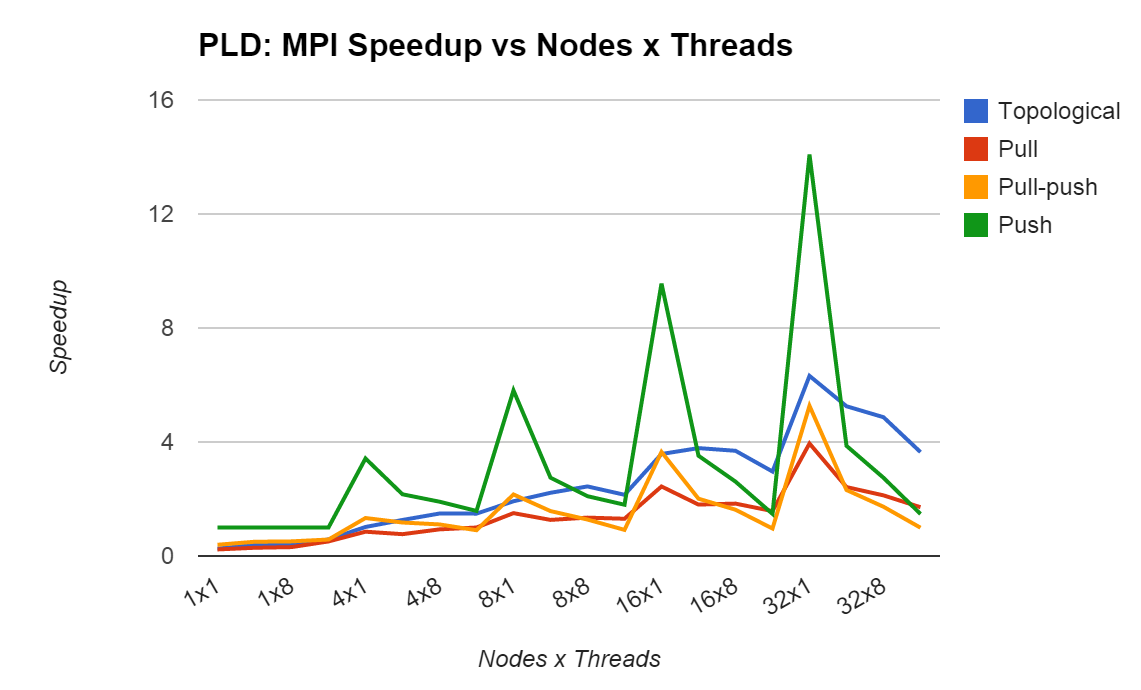
\includegraphics[width=.99\linewidth]{PLDMPISpeedup}
  \caption{PLD}
  \label{fig:ftime}
\end{subfigure}
\caption{Speedup over MPI nodes of different PageRank implementations on datasets from table~\ref{table:data}}
\label{fig:spMPI}
\end{figure}

The general trends in performance as seen in~\ref{fig:time}, are that the Pull and Pull-push implementations are generally the slowest, and the Push and Topological implementations are inconsistently \#1 and \#2 in speed. This performance can be due to a number of things such as:

\
message vs nodes trade off, parallelizability of each algorithm, and computational overhead for each algorithm. 




\subsection{ADMM Results Compared to other Linear methods}
The results below are an attempt to compare other parallel linear solvers for Ax=b  on different data sets and machines with our results for ADMM. This is not the primary focuse of the ADMM results, but it may offer some general intuition about the ADMM method compared to linear solvers not addressed in this paper.
The residual value, after which the process stops, for all data below was set to $10^{-7}$ and the data set used for the ADMM method was the livejournal dataset.
\begin{center}
  \begin{tabular}{c|c|c|c|c}
	\hline
	Method & Nodes & Iterations & Total Time (s) & Processes \\
	\hline\hline
	Jacobi & 300M & 71 & 9.94 & 60\\
	PR & 14M & 84  & 5.04 & 20 \\ 
	ADMM & 83.6M & 345 & 38.8  & 16 \\
	ADMM & 83.6M & 643 & 28.15 & 64 \\
  \end{tabular}
\end{center}

Again, although it is difficult to compare results on different data sets from different machines, the above results would indicate that the ADMM method (with gradient descent minimization) does not perform well compared to other parallel methods. This poor performance is likely due to a few things: As we increase the number of processes to solve the problem, the amount of information that has to be passed through MPI becomes a bigger burden and this ADMM code has not been optimized for message passing. Also, the minimization solver could likely be improved by changing the solver to something that is more appropriate given the underdetermined systems that are solved. Our ADMM solver, unlike our data-drive approach, does not take into consideration any information about the structure or values of our data. It would be possible to optimize according to some update criteria; this will be exapnded upon in the future work section of this paper. Also, the software used in the competing methods (PETSC) has been significantly optimized and therefore we generally should expect our naive method to peform worse, regardless of the specific solver.
\newline
\linebreak
In addition to comparing the ADMM method to other parallel (Ax=b) solvers, the data set below will serve as a way to compare ADMM to the power iteration methods (push, pull, push-pull, topological). The DataSet column below will indicate the livejournal(LJ) or friendster(FR). We chose to not run the ADMM method on any larger data sets as the results for this method tended to be poor and the primary purpose of this paper is to focus on the results of distributing the data-driven methods.

\begin{center}
  \begin{tabular}{c|c|c|c}
	\hline
	DataSet & Iterations & Total Time (s) & Processes \\
	\hline\hline
	LJ & 345 & 38.8  & 16 \\
	LJ & 643 & 28.15 & 64 \\
	LJ & 1043 & 36.2 & 128 \\
	FR &  &  & 16 \\
	FR &  &  & 64 \\
	FR &  &  & 128 \\
  \end{tabular}
\end{center}
The results above would indicate that there is the expected speed up when we increase the number of processes, but it is without question not a linear speed up. Again, we suspect this is due to the increase in message overhead. It is also indicated that the time per iteration increases which is exactly what we expected. Each iteration should take less time as the amount of data on each process will decrease with an increase in processes. Additionally, the number of iterations increases which we also expected since each individual process has an underdetermined process and will quickly solve for some minimum value but may not be close to the final global solution (dues to many local minimums) and therefore require much guidance (updates from the global variable z) to converge. Finally, we notice that with 128 processes, the total solve time begins to increase. We suspect this again due to inefficient message passing consuming a significant amount of time.
\newline
\pagebreak
Although ADMM appeared to have poor results relative to other tested methods, it should be noted that the coding for ADMM was relatively simple and easy to understand. Aside from getting familiar with MPI and the minimzation solver, there was nothing difficult about creating the code. A valuable metric for those looking for a quick (not so efficient) method for solving problems in this category.

\section{Future Work}
Related to ADMM, there are many possible areas to focus for future research. Optimization can be done around selecting a better method for minimzation on each process. Not only around the general method, but modifying that method to take a more data-driven approach since we have seen this can have a significant impact on results. Our approach uses the lasso method ($L^{1}$) regularization with the intent to creat a sparse solution therefore reducing message overhead if using a sparse matrix/vector representation, which proved to be less efficient than standard solvers. 
\newline
Aside from updating the minimization solver, the ADMM method could be improved by optimizing the message passing process. The curent code does not take into consideration sparsity of data nor the change in values it updates; meaning if a values was being updated to a values that was not significanlty different than its original value, can there be significant speed up with deciding not to update those values. This could be tremendously valuable when updating the global value z and broadcasting that update back to all processes.

\section{Conclusion}

\vfill\pagebreak
\bibliographystyle{IEEEbib}
\bibliography{refs}


%\begin{thebibliography}{1}

%\bibitem{PowerLawGraphs} David Gleich, et al. {\em Scalable Computing for Power Law Graphs: Experience with Parallel PageRank}

%\bibitem{FastParallel} David Gleich, et al. {\em Fast Parallel PageRank: A Linear System Approach} 

%\bibitem{ADMM} Stephen Boyd, et al. {\em Distributed Optimization and Statistical Learning via the Alternating Direction Method of Multipliers} 

%\bibitem{Joyce} Joyce Whang, et al. {\em Scalable Data-driven PageRank: Algorithms, System Issues '\&' Lessons Learned}
 
 %\bibitem{MPIref} mcs.anl.gov {\em http://www.mcs.anl.gov/research/projects/mpi/tutorial/mpiexmpl/src/jacobicmpl/C/main.html}
 
 %\bibitem{FSU} fsu.edu {\em http://people.sc.fsu.edu/~jburkardt/cppsrc/mpi/mpi.html}

% \bibitem{MPIPR} Xiaoyi (Eric) Li  {\em Parallel PageRank Computation using MPI}

% \bibitem{YahooPPR} David Gleich, Leonid Zhukov, Pavel Berkhin  {\em Fast Parallel PageRank: Methods and Evaluations}

 %\bibitem{IndianaPPR} Shubhada Karavinkoppa and Jayesh Kawli  {\em Page Rank Algorithm Using MPI}

 %\bibitem{MixedMPI} Bundit Manaskasemsak, Putchong Uthayopas, Arnon Rungsawang {\em A Mixed MPI-Thread Approach for Parallel Page Ranking Computation}

%\end{thebibliography}

\end{document}
